\documentclass[12pt, a4paper]{book}

\usepackage[T1]{fontenc}
\usepackage[utf8]{inputenc}
\usepackage[charter, cal=cmcal]{mathdesign}
\usepackage[scaled=0.92]{helvet}
\usepackage{geometry}
\geometry{a4paper, top=30mm, bottom=30mm, inner=32mm, outer=25mm, marginparwidth=18mm}

\usepackage{amsmath, amsthm}
\usepackage[version=4]{mhchem}
\usepackage{graphicx}
\usepackage{xcolor}
\usepackage{tikz}
\usetikzlibrary{arrows.meta, shapes.geometric, positioning, calc, backgrounds}
\usepackage{pgfplots}
\pgfplotsset{compat=1.18}
\usepackage{tcolorbox}
\tcbuselibrary{skins, breakable, theorems}
\usepackage{titlesec}
\usepackage{fancyhdr}
\usepackage{enumitem}
\usepackage{booktabs}
\usepackage{array}
\usepackage{parskip}
\usepackage{siunitx}
\usepackage[colorlinks=true, linkcolor=BrickRed,
            urlcolor=NavyBlue, citecolor=ForestGreen]{hyperref}

% ── Colours (Journey 8 — forest green / amber) ────────────────────────────────
\definecolor{JourneyColor}{HTML}{065F46}
\definecolor{ModuleColor}{HTML}{059669}
\definecolor{PuzzleColor}{HTML}{B45309}
\definecolor{DiscoveryColor}{HTML}{D97706}
\definecolor{WarningColor}{HTML}{991B1B}
\definecolor{ProblemColor}{HTML}{6B21A8}
\definecolor{ReflectColor}{HTML}{0D9488}
\definecolor{HistoryColor}{HTML}{78350F}

% ── Boxes ─────────────────────────────────────────────────────────────────────
\newtcolorbox{puzzlebox}[1][]{enhanced,breakable,
  colback=PuzzleColor!6,colframe=PuzzleColor,fonttitle=\bfseries\sffamily,
  title={The Puzzle},attach boxed title to top left={yshift=-2mm,xshift=6mm},
  boxed title style={colback=PuzzleColor},borderline west={3pt}{0pt}{PuzzleColor},#1}

\newtcolorbox{discoverybox}[1][]{enhanced,breakable,
  colback=DiscoveryColor!8,colframe=DiscoveryColor,fonttitle=\bfseries\sffamily,
  title={Discovery},attach boxed title to top left={yshift=-2mm,xshift=6mm},
  boxed title style={colback=DiscoveryColor},borderline west={3pt}{0pt}{DiscoveryColor},#1}

\newtcolorbox{problembox}[1][]{enhanced,breakable,
  colback=ProblemColor!5,colframe=ProblemColor,fonttitle=\bfseries\sffamily,
  title={Problems},attach boxed title to top left={yshift=-2mm,xshift=6mm},
  boxed title style={colback=ProblemColor},borderline west={3pt}{0pt}{ProblemColor},#1}

\newtcolorbox{deepbox}[1][]{enhanced,breakable,
  colback=JourneyColor!5,colframe=JourneyColor,fonttitle=\bfseries\sffamily,
  title={Deep Problems},attach boxed title to top left={yshift=-2mm,xshift=6mm},
  boxed title style={colback=JourneyColor},borderline west={4pt}{0pt}{JourneyColor},#1}

\newtcolorbox{historybox}[1][]{enhanced,breakable,
  colback=HistoryColor!7,colframe=HistoryColor!60,fonttitle=\bfseries\sffamily\small,
  title={Historical Note},attach boxed title to top left={yshift=-2mm,xshift=6mm},
  boxed title style={colback=HistoryColor!80},#1}

\newtcolorbox{reflectionbox}[1][]{enhanced,breakable,
  colback=ReflectColor!6,colframe=ReflectColor,fonttitle=\bfseries\sffamily,
  title={Reflection},attach boxed title to top left={yshift=-2mm,xshift=6mm},
  boxed title style={colback=ReflectColor},borderline west={3pt}{0pt}{ReflectColor},#1}

\newtcolorbox{namedconcept}[2][]{enhanced,
  colback=ModuleColor!6,colframe=ModuleColor,fonttitle=\bfseries\sffamily\large,
  title={#2},attach boxed title to top left={yshift=-2mm,xshift=6mm},
  boxed title style={colback=ModuleColor},#1}

% ── Section formatting ────────────────────────────────────────────────────────
\titleformat{\chapter}[display]
  {\normalfont\sffamily\huge\bfseries\color{JourneyColor}}
  {\textcolor{JourneyColor!60}{\chaptertitlename\ \thechapter}}{10pt}{\Huge}
  [\vspace{2pt}\textcolor{JourneyColor}{\titlerule[1.5pt]}]
\titleformat{\section}
  {\normalfont\sffamily\Large\bfseries\color{ModuleColor}}
  {\thesection}{1em}{}[\textcolor{ModuleColor!40}{\titlerule[0.6pt]}]
\titleformat{\subsection}
  {\normalfont\sffamily\large\bfseries\color{JourneyColor!80}}{\thesubsection}{1em}{}
\titleformat{\subsubsection}
  {\normalfont\sffamily\normalsize\bfseries}{\thesubsubsection}{1em}{}

\pagestyle{fancy}
\fancyhf{}
\fancyhead[LE]{\small\sffamily\textcolor{JourneyColor}{\leftmark}}
\fancyhead[RO]{\small\sffamily\textcolor{ModuleColor}{\rightmark}}
\fancyfoot[C]{\small\thepage}
\renewcommand{\headrulewidth}{0.4pt}

\newcommand{\newterm}[1]{\textit{\textcolor{DiscoveryColor}{#1}}}
\newcommand{\important}[1]{\textcolor{ModuleColor}{\textbf{#1}}}

\begin{document}

\setcounter{chapter}{7}
\chapter[Journey 8 --- Materials and Solid-State Chemistry]
        {Journey Eight\\[8pt]
         \textcolor{ModuleColor}{\large Materials and Solid-State Chemistry}}
\setcounter{section}{0}

\section{Module 8.1 --- Band Theory of Solids}
\label{sec:mod8.1}

\subsection*{Motivation}

We completed in Journey 7 the biophysical track of organic chemistry, studying how molecular structures drive biological life.
Now, we transition to the solid state.

In traditional chemistry, we study isolated molecules in gas or liquid phases.
But when atoms assemble into an infinite crystalline solid, their individual atomic orbitals overlap to form macroscopic networks.
This infinite extension of molecular orbital theory is **Band Theory**.
By analyzing how orbital splitting divides the electronic states of solids, we discover why some materials conduct electricity freely, others act as barriers, and a unique class—semiconductors—can be controlled to drive the logic of computer chips.

\subsection{The Diamond-Silicon Divergence}

We investigate how Group 14 elements with identical structures exhibit completely different electric properties.

\begin{puzzlebox}
\textbf{The Conductive Anomaly.}

Diamond and Silicon are in the same group of the periodic table (Group 14). Both possess four valence electrons, hybridize to $sp^3$, and crystallize into the exact same face-centered cubic lattice known as the diamond cubic structure.
\begin{enumerate}[label=(a), leftmargin=*]
  \item Diamond is completely transparent to visible light and is a near-perfect electrical insulator, blocking all electric current.
        Silicon, however, has a dark, shiny metallic luster and behaves as a semiconductor, allowing a controlled flow of charge.
        Why do two materials containing group-equivalent atoms, with the same orbital hybridization and same crystal structure, display such different electrical properties?
  \item In molecular orbital theory, when two orbitals combine, they split into a bonding orbital (lower energy) and an anti-bonding orbital (higher energy).
        As we assemble $N$ atoms in a solid lattice (where $N \to 10^{23}$), what happens to this orbital splitting? (How does the spacing between the $N$ resulting energy levels change?)
  \item This infinite splitting forms continuous **energy bands**.
        Identify the **valence band** (the band filled with valence electrons) and the **conduction band** (the empty band above it). What is the name of the energy gap between them?
\end{enumerate}
\end{puzzlebox}

\subsection{Insulators, Metals, and Semiconductors}

We classify materials based on the size of their band gaps and the availability of charge carriers.

\begin{explobox}
We classify solid materials into three categories based on their electronic band structure:
1. **Metals:** No band gap; the valence and conduction bands overlap, or the valence band is only partially filled. Electrons can move freely under a voltage.
2. **Insulators:** A large band gap ($E_g > \SI{3}{eV}$). The thermal energy at room temperature is far too small to promote electrons.
3. **Semiconductors:** A small band gap ($E_g \approx \SI{0.5}{eV}$ to $\SI{2.0}{eV}$). A fraction of electrons can be thermally promoted, leaving behind positive vacancies called **holes**.

\begin{center}
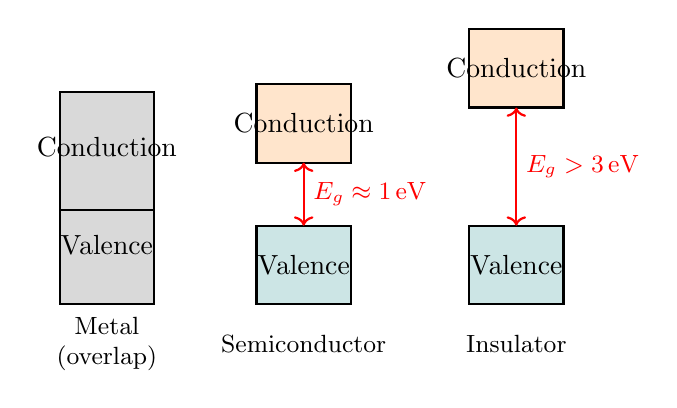
\begin{tikzpicture}[scale=1.0]
  % Metal
  \draw[fill=gray!30, thick] (0,0) rectangle (1.2,1.5);
  \draw[fill=gray!30, thick] (0,1.2) rectangle (1.2,2.7);
  \node at (0.6,0.75) {Valence};
  \node at (0.6,2.0) {Conduction};
  \node[align=center, font=\small] at (0.6,-0.5) {Metal\\(overlap)};
  
  % Semiconductor
  \begin{scope}[xshift=2.5cm]
    \draw[fill=teal!20, thick] (0,0) rectangle (1.2,1.0);
    \draw[fill=orange!20, thick] (0,1.8) rectangle (1.2,2.8);
    \draw[<->, red, thick] (0.6,1.0) -- (0.6,1.8);
    \node[right, red, font=\small] at (0.6,1.4) {$E_g \approx \SI{1}{eV}$};
    \node at (0.6,0.5) {Valence};
    \node at (0.6,2.3) {Conduction};
    \node[align=center, font=\small] at (0.6,-0.5) {Semiconductor};
  \end{scope}
  
  % Insulator
  \begin{scope}[xshift=5.2cm]
    \draw[fill=teal!20, thick] (0,0) rectangle (1.2,1.0);
    \draw[fill=orange!20, thick] (0,2.5) rectangle (1.2,3.5);
    \draw[<->, red, thick] (0.6,1.0) -- (0.6,2.5);
    \node[right, red, font=\small] at (0.6,1.75) {$E_g > \SI{3}{eV}$};
    \node at (0.6,0.5) {Valence};
    \node at (0.6,3.0) {Conduction};
    \node[align=center, font=\small] at (0.6,-0.5) {Insulator};
  \end{scope}
\end{tikzpicture}
\end{center}
\begin{enumerate}[label=(\alph*), leftmargin=*]
  \item Silicon has a band gap of $E_g = \SI{1.12}{eV}$. Diamond has a band gap of $E_g = \SI{5.50}{eV}$.
        Explain the Diamond-Silicon divergence in terms of these values.
  \item Why does a semiconductor's electrical conductivity *increase* as the temperature rises, whereas a metal's conductivity *decreases*? (Consider the thermal generation of carriers vs. lattice vibrations scattering the electrons).
\end{enumerate}
\end{explobox}

\subsection{Direct vs. Indirect Band Gaps}

We examine the momentum space constraints that govern optical transitions in materials.

\begin{explobox}
In solid-state physics, electron states in a crystal are indexed by their wave vector $k$ (crystal momentum).
* **Direct Band Gap:** The maximum of the valence band and the minimum of the conduction band occur at the same wave vector $k$. An electron can transition by absorbing or emitting a photon without changing momentum.
* **Indirect Band Gap:** The maximum and minimum occur at different wave vectors. A transition requires both a photon and a lattice vibration particle (**phonon**) to conserve both energy and momentum.
\begin{enumerate}[label=(\alph*), leftmargin=*]
  \item Why are direct band gap semiconductors (like gallium arsenide, GaAs) highly efficient at emitting light, making them ideal for laser diodes and LEDs, whereas indirect band gap semiconductors (like silicon) are extremely poor light emitters?
  \item If a silicon crystal absorbs a photon of energy $h\nu > E_g$, where does the excess energy go? (What happens to the momentum mismatch?)
\end{enumerate}
\end{explobox}

\newpage

% ─── Section: Discovery ──────────────────────────────────────────────────────
\section{Part 3 --- Discovery}

\begin{discoverybox}
\textbf{What have we built?}

\textbf{First.} Band theory is the infinite extension of molecular orbital theory: $10^{23}$ overlapping atomic orbitals form continuous energy bands separated by a band gap ($E_g$).

\textbf{Second.} The size of the band gap divides materials into metals ($E_g = 0$), semiconductors ($E_g \approx \SI{1}{eV}$), and insulators ($E_g > \SI{3}{eV}$).

\textbf{Third.} Thermal promotion of electrons from the valence band to the conduction band generates charge carriers: free electrons and positive holes, making semiconductor conductivity highly temperature-dependent.

\textbf{Fourth.} Direct band gaps allow efficient, single-photon optical transitions. Indirect band gaps require a phonon to conserve momentum, making optical transitions much slower and non-radiative.
\end{discoverybox}

\newpage

% ─── Section: Naming Concepts ────────────────────────────────────────────────
\section{Part 4 --- What This Is Called}

\begin{namedconcept}{Solid-state parameters}
* **Valence Band:** The highest energy band that is completely filled with electrons at absolute zero.
* **Conduction Band:** The lowest energy band that is vacant at absolute zero, into which electrons can be promoted to conduct current.
* **Band Gap ($E_g$):** The forbidden energy region between the valence and conduction bands where no electron states can exist.
* **Hole:** The positive charge carrier created when an electron is promoted out of the valence band, representing a vacant state that can move through the lattice.
* **Direct Band Gap:** A band structure where the valence band maximum and conduction band minimum align in momentum space ($k$-space).
\end{namedconcept}

\newpage

% ─── Section: Solved Exercises ───────────────────────────────────────────────
\section{Part 5 --- Solved Exercises}

\begin{problembox}
\begin{enumerate}[label=\textbf{E\arabic*.}]
  \item \textbf{Light Absorption Threshold.}
  
        Calculate the maximum (threshold) wavelength of light $\lambda$ (in nm) required to promote an electron across the band gap of silicon ($E_g = \SI{1.12}{eV}$).
        
        \textbf{Solution:}
        For a photon to promote an electron across the band gap, its energy must be greater than or equal to $E_g$:
        \[
          E \;=\; \frac{h c}{\lambda} \;\ge\; E_g \implies \lambda_{\text{max}} \;=\; \frac{h c}{E_g}.
        \]
        Here:
        * $h \approx 6.626 \times 10^{-34}$ J$\cdot$s (Planck's constant).
        * $c \approx 3.000 \times 10^8$ m/s (speed of light).
        * $E_g = \SI{1.12}{eV} = 1.12 \times 1.602 \times 10^{-19}$ J $= 1.794 \times 10^{-19}$ J.
        
        Substitute these values:
        \[
          \lambda_{\text{max}} \;=\; \frac{\left( 6.626 \times 10^{-34} \text{ J}\cdot\text{s} \right) \left( 3.000 \times 10^8 \text{ m/s} \right)}{1.794 \times 10^{-19} \text{ J}}.
        \]
        Evaluate the product in the numerator:
        \[
          h c \;=\; 1.988 \times 10^{-25} \text{ J}\cdot\text{m}.
        \]
        Calculate the wavelength:
        \[
          \lambda_{\text{max}} \;=\; \frac{1.988 \times 10^{-25}}{1.794 \times 10^{-19}} \;=\; 1.108 \times 10^{-6} \text{ m} \;=\; 1108 \text{ nm}.
        \]
        Thus, the maximum wavelength is \SI{1108}{nm}, which lies in the near-infrared region of the spectrum.
        Any light with a wavelength shorter than \SI{1108}{nm} (which includes all visible light) can be absorbed by silicon, explaining why silicon solar cells absorb sunlight so efficiently.
        
  \item \textbf{1D Density of States near a Band Edge.}
  
        In solid-state physics, the energy-momentum relation for electrons near a 1D band edge is quadratic:
        \[
          E(k) \;=\; \frac{\hbar^2 k^2}{2m^*},
        \]
        where $m^*$ is the effective mass of the electron.
        Prove that the density of states $g(E)$ in 1D scales as $g(E) \propto E^{-1/2}$.
        
        \textbf{Solution:}
        By definition, the density of states in 1D is related to the derivative of the number of states with respect to energy:
        \[
          g(E) \;=\; \frac{dN}{dE} \;=\; \frac{dN}{dk} \cdot \frac{dk}{dE}.
        \]
        In 1D, the number of states in $k$-space is proportional to $k$: $N(k) \propto k \implies \frac{dN}{dk} = \text{constant}$.
        To find $\frac{dk}{dE}$, we solve the energy relation for $k$:
        \[
          k \;=\; \sqrt{\frac{2m^* E}{\hbar^2}} \;=\; \left(\frac{2m^*}{\hbar^2}\right)^{1/2} E^{1/2}.
        \]
        Differentiate $k$ with respect to $E$:
        \[
          \frac{dk}{dE} \;=\; \left(\frac{2m^*}{\hbar^2}\right)^{1/2} \frac{1}{2} E^{-1/2}.
        \]
        Substitute this back:
        \[
          g(E) \;\propto\; \frac{dk}{dE} \;\propto\; E^{-1/2}.
        \]
        This completes the proof. Note that this density of states diverges as $E \to 0$ (the band edge), a phenomenon called a **van Hove singularity**, which has massive consequences for the conductivity of 1D quantum wires.
\end{enumerate}
\end{problembox}

\newpage

% ─── Section: Problems ───────────────────────────────────────────────────────
\section{Part 6 --- Problems}

\begin{problembox}
\begin{enumerate}[label=\textbf{P\arabic*.}]
  \item \textbf{Carrier Concentration and Temperature.}
  
        The concentration of thermally promoted electrons in the conduction band of an intrinsic semiconductor is given by:
        \[
          n_i \;=\; C \cdot T^{3/2} e^{-\frac{E_g}{2 k_B T}},
        \]
        where $C$ is a material constant and $k_B \approx 8.617 \times 10^{-5}$ eV$\cdot$K$^{-1}$ is the Boltzmann constant.
        \begin{enumerate}[label=(\alph*)]
          \item Calculate the exponential term $e^{-E_g / 2k_B T}$ at $T = \SI{298}{K}$ for:
                * Silicon: $E_{g} = 1.12$ eV.
                * Diamond: $E_{g} = 5.50$ eV.
          \item Compare the ratio $n_{i,\text{Silicon}}/n_{i,\text{Diamond}}$ at room temperature.
          \item If we heat diamond to $T = \SI{1000}{K}$, calculate its new exponential term. Does diamond behave as a semiconductor at high temperatures?
        \end{enumerate}

  \item \textbf{LED Color Engineering.}
  
        A light-emitting diode (LED) emits light when an electron recombines with a hole across a direct band gap, releasing a photon of energy $h\nu \approx E_g$.
        Calculate the required band gap $E_g$ (in eV) to construct:
        \begin{enumerate}[label=(\alph*)]
          \item A red LED emitting at $\lambda = \SI{650}{nm}$.
          \item A blue LED emitting at $\lambda = \SI{450}{nm}$.
        \end{enumerate}
\end{enumerate}
\end{problembox}

\newpage

% ─── Section: Deep Problems ──────────────────────────────────────────────────
\section{Part 7 --- Deep Problems}

\begin{deepbox}
\begin{enumerate}[label=\textbf{D\arabic*.}]
  \item \textbf{The Kronig-Penney Model.}
  
        We model a 1D solid as a periodic array of delta-function potential barriers representing the nuclei:
        \[
          V(x) \;=\; \sum_{n=-\infty}^\infty V_0 \delta(x - na).
        \]
        By Bloch's Theorem, the wave function of an electron in a periodic potential has the form $\psi(x) = u(x) e^{i k x}$, where $u(x + a) = u(x)$, and $k$ is the wave vector.
        Solving the Schrödinger equation for this periodic potential yields the transcendental relation:
        \[
          P \frac{\sin \alpha a}{\alpha a} + \cos \alpha a \;=\; \cos ka,
        \]
        where $\alpha = \sqrt{\frac{2mE}{\hbar^2}}$, and $P = \frac{m V_0 a}{\hbar^2}$ represents the barrier strength.
        \begin{enumerate}[label=(\alph*)]
          \item The wave vector $k$ must be real for a state to represent a physically propagating electron. Explain why this requires:
          \[
            -1 \;\le\; P \frac{\sin \alpha a}{\alpha a} + \cos \alpha a \;\le\; 1.
          \]
          \item Let $P = 3$. Plot the function $f(\alpha a) = 3 \frac{\sin \alpha a}{\alpha a} + \cos \alpha a$ versus $\alpha a$.
                Highlight the regions where $|f(\alpha a)| > 1$.
          \item Explain why these forbidden regions correspond to **band gaps**, whereas the regions with $|f(\alpha a)| \le 1$ correspond to **energy bands**.
          \item Show that if $P \to 0$ (free electrons), the energy spectrum is continuous. Show that if $P \to \infty$ (isolated atoms), the spectrum becomes discrete.
        \end{enumerate}

  \item \textbf{Indirect Transitions and Phonons.}
  
        Silicon is an indirect semiconductor. The valence band maximum occurs at $k = 0$, but the conduction band minimum occurs at $k \approx 0.85 \frac{\pi}{a}$ (near the edge of the Brillouin zone).
        \begin{enumerate}[label=(\alph*)]
          \item Explain why an electron cannot absorb a photon of energy $E = E_g$ directly to jump across this gap. (Consider the momentum of a photon $p_{\text{photon}} = h/\lambda$ compared to the crystal momentum difference $\Delta p = \hbar \Delta k \approx 0.85 \frac{\hbar\pi}{a}$, where $a \approx \SI{5.43}{\text{\AA}}$).
          \item A phonon is a quantized lattice vibration. It carries significant momentum but very little energy (typical phonon energy is only $\sim \SI{0.03}{eV}$).
                Explain how the cooperative absorption of a photon and a phonon allows silicon to undergo this indirect transition.
        \end{enumerate}
\end{enumerate}
\end{deepbox}

\newpage

% ─── Section: Reflection ─────────────────────────────────────────────────────
\section{Part 8 --- Reflection}

\begin{reflectionbox}
\textbf{Conceptual Reflection}

Consider the following questions:
\begin{enumerate}
  \item **On the Infinite Limit:** Band theory is based on the assumption of an infinite, perfect periodic crystal lattice. But all real solid samples are finite and contain surface boundaries and defects. Why does the band structure approximation still work so exceptionally well for macroscopic solids?
  \item **On Group 14 Trends:** As you move down Group 14 (Carbon $\to$ Silicon $\to$ Germanium $\to$ Tin $\to$ Lead), the band gap decreases: $E_{g,\text{Diamond}} = 5.5$ eV, $E_{g,\text{Si}} = 1.1$ eV, $E_{g,\text{Ge}} = 0.7$ eV, $E_{g,\text{Sn}} = 0.1$ eV, and Lead is a metal. Why does the band gap shrink as the atomic number increases? (Consider the size of the orbitals and the strength of the overlap).
  \item **On Symmetries:** The Kronig-Penney model shows that translational symmetry (periodicity) is the physical source of energy bands and band gaps. Does this mean that the electronic properties of materials are ultimately properties of geometric symmetry?
\end{enumerate}
\end{reflectionbox}

\medskip
\noindent\textbf{Looking ahead.}
Module~8.2 introduces **Silicon Doping and Semiconductors**. Having established how bands form, we will study how to control their conductivity by adding trace amounts of impurities (doping). We will explore n-type and p-type materials, and discover the physics of the p-n junction.

\vspace{1.4cm}
\begin{center}
{\color{JourneyColor}\rule{0.5\linewidth}{0.8pt}}\\[6pt]
{\small\color{JourneyColor}\textit{End of Journey 8, Module 8.1 --- Band Theory of Solids}}\\[4pt]
{\small\color{JourneyColor}Continue to: \textbf{Module 8.2 --- Silicon Doping and Semiconductors}}\\[6pt]
{\color{JourneyColor}\rule{0.5\linewidth}{0.8pt}}
\end{center}

\end{document}
